% !TeX program = pdfLaTeX
\documentclass[12pt]{article}
\usepackage{amsmath}
\usepackage{amsthm}
\usepackage{graphicx,psfrag,epsf}
\usepackage{enumerate}
%\usepackage[numbers]{natbib}
\usepackage[nomarkers]{endfloat}
\usepackage{natbib}
\setcitestyle{numbers} 
\makeatletter % Reference list option change
\renewcommand\@biblabel[1]{#1. } % from [1] to 1
\makeatother %

\usepackage{booktabs}
\usepackage{longtable}
\usepackage{array}
\usepackage{adjustbox}
\usepackage{multirow}
\usepackage{subfig}
\usepackage[table,xcdraw]{xcolor}
\usepackage{wrapfig}
\usepackage{float}
%\usepackage{colortbl}
\usepackage[colorlinks]{hyperref}
\hypersetup{
  colorlinks=true,
  citecolor=black,
  linkcolor=black,
  urlcolor=blue}
  
\usepackage{pdflscape}
\usepackage{tabu}
\usepackage{threeparttable}
\usepackage{url} % not crucial - just used below for the URL

\usepackage{etoolbox}% http://ctan.org/pkg/etoolbox
\makeatletter
\patchcmd{\subsection}{\bfseries}{\relax}{}{}% Non-bold \subsection
\patchcmd{\subsubsection}{\bfseries}{\relax}{}{}% Non-bold \subsection
\makeatother


%\pdfminorversion=4
% NOTE: To produce blinded version, replace "0" with "1" below.
\newcommand{\blind}{}

% DON'T change margins - should be 1 inch all around.
\addtolength{\oddsidemargin}{-.5in}%
\addtolength{\evensidemargin}{-.5in}%
\addtolength{\textwidth}{1in}%
\addtolength{\textheight}{1.3in}%
\addtolength{\topmargin}{-.8in}%

\newenvironment{definition}[1]% environment name 
{% begin code 
  \par\vspace{.75\baselineskip}\noindent 
  \textbf{Definition (#1)}\begin{itshape}% 
  \par\vspace{.5\baselineskip}\noindent\ignorespaces 
}% 
{% end code 
  \end{itshape}\ignorespacesafterend 
}

\providecommand{\tightlist}{%
  \setlength{\itemsep}{0pt}\setlength{\parskip}{0pt}}

\begin{document}

\def\spacingset#1{\renewcommand{\baselinestretch}%
{#1}\small\normalsize} \spacingset{1}


%%%%%%%%%%%%%%%%%%%%%%%%%%%%%%%%%%%%%%%%%%%%%%%%%%%%%%%%%%%%%%%%%%%%%%%%%%%%%%

\if0\blind
{
  \title{\bf A Robust Approach to Automatic Groove Identification in 3D Bullet Land
Scans}

  \author{
        \\ %\\
    \\
    % \\
      }
    \maketitle
  \bigskip
  \begin{center}
  {
  \textbf{Affiliation(s)}\\
  Department of Statistics, Iowa State University and CSAFE (Center for
  Statistics and Applications in Forensic Evidence)\\
  \bigskip
  \textbf{Source of funding}\\
  \\
  \bigskip
  \textbf{Acknowledgement}\\
  \\
  \bigskip
  \textbf{Information on presentation of work}\\
  
  }
  \end{center}

} \fi

  % \bigskip

  % \bigskip
\newpage

\if0\blind
{
  \bigskip
  \bigskip
  \bigskip
  \begin{center}
  \title{\LARGE\bf A Robust Approach to Automatic Groove Identification in 3D Bullet Land
Scans}
  \end{center}
  \bigskip
  \maketitle
} \fi


\bigskip
\begin{abstract}

\end{abstract}

\noindent%
{\it Keywords:} 
\vfill

\newpage
\spacingset{1.45} % DON'T change the spacing!

\section{Background}

For years, forensic firearms examiners have analyzed bullet striations
through a process of visual feature comparison to determine whether two
patterns are in sufficient agreement \citep{AFTE}. Examiners compare
striation marks on land engraved areas of a bullet fired from a known
barrel to a questioned bullet when investigating whether both bullets
were propelled through the same gun barrel.

These visual analyses are one of several feature comparison methods
whose scientific foundations were questioned in the 2009 report by the
National Research Council on Identifying the Needs of the Forensic
Sciences Community \citep{NRC2009}.

Following that 2009 report, researchers began more intensely studying
the validity of feature comparison methods as well as investigating the
feasibility of developing image-analysis algorithms to complete
automated, quantitative analyses. The main technological development
that has created a pathway for image-analysis techniques is the
introduction of high resolution 3D scanning technology to the field of
forensic science.

3D scanning technology not only allows for preservation of current and
historical evidence in digital format, it also provides extremely
detailed representations of forensically relevant portions of fired
bullets. In recent years, this technology has been applied to the
collection of topological images of both bullet lands and breech faces
\citep[e.g.][]{DeKinder1, DeKinder2, Bachrach1}. These 3D data have
since been used in the development of several methods of varying
complexity for automated comparison of land engraved areas
\citep[e.g.][]{Ma1, Chu1, Chu2, Hare1}.

Criticisms of firearms examination in recent years have focused on
foundational validity and reliability \citep[e.g.][]{PCAST2016}. These
criticisms enforce the need for automated algorithms to undergo careful
study and validation before they can be reasonably implemented to assist
forensic firearms examiners. This process of algorithm development
includes data pre-processing methods that ensure the correct data are
being used in automated methods.

Data pre-processing is not usually considered a significant barrier for
most research endeavors. However, the nature of the 3D scanning process
for land engraved areas (LEAs) introduces a challenging data
pre-processing problem. To guarantee capture of an entire land engraved
area, scanning across the object must begin and end in the neighboring
groove engraved areas (GEAs). This ensures that the maximal amount of
land surface area can be utilized in image-analysis methods, providing
the most reliable feature generation and more robust results. This
extraneous data collection, while necessary, dictates the most
significant step in data pre-processing: correctly identifying between
data from LEAs and GEAs.

Dealing with these two areas separately is crucial to ensure accuracy
and precision in subsequent processing steps. Removal of data from
groove engraved areas significantly reduces the possibility of
misidentification of the characteristics used in automated comparisons.
In order to distinguish between these areas, we aim to identify
``shoulder locations'', the locations at which the LEA ends and the GEAs
begin.

Distinguishing between land and groove engraved areas is a problem at
which human vision excels, but it is quite challenging for automatic
procedures due to the nature of the data collected: the bullet curvature
presents the main structure in the data, but the abrupt change between
land and groove engraved areas introduces a competing structure. The
atypical structure overwhelms standard statistical modeling techniques
which cannot distinguish between the structures. An early solution based
on data smoothing (described in \citep{Hare1}) can result in
misidentification of deep striae as shoulder locations. The following
work describes a better solution to this pre-processing problem based on
robust statistical methods.

\section{Data Source}

The data used in this paper are high resolution 3D scans of 208 bullet
land engraved areas. The scanned bullets come from Hamby Set 44
\citep{Hamby}. They consist of 35 total bullets from a set of 10
consecutively rifled Ruger P85 barrels. These LEAs were scanned at Iowa
State University's High Resolution Microscopy Facility, and the scans
are stored in 3D format as x3p files, conforming to the ISO5436-2
standard \textbf{cite ISO standard from sourceforge here??}. The data,
seen in Figure 1, are gathered at a resolution of .645 microns per
pixel. Physically, each land is approximately 2 millimeters in width.
With a .645 micron per pixel resolution, data structures can contain
more than 3 million individual data points. The 35 total bullets with 6
lands per bullet result in 210 individual lands.

\begin{figure}
\centering
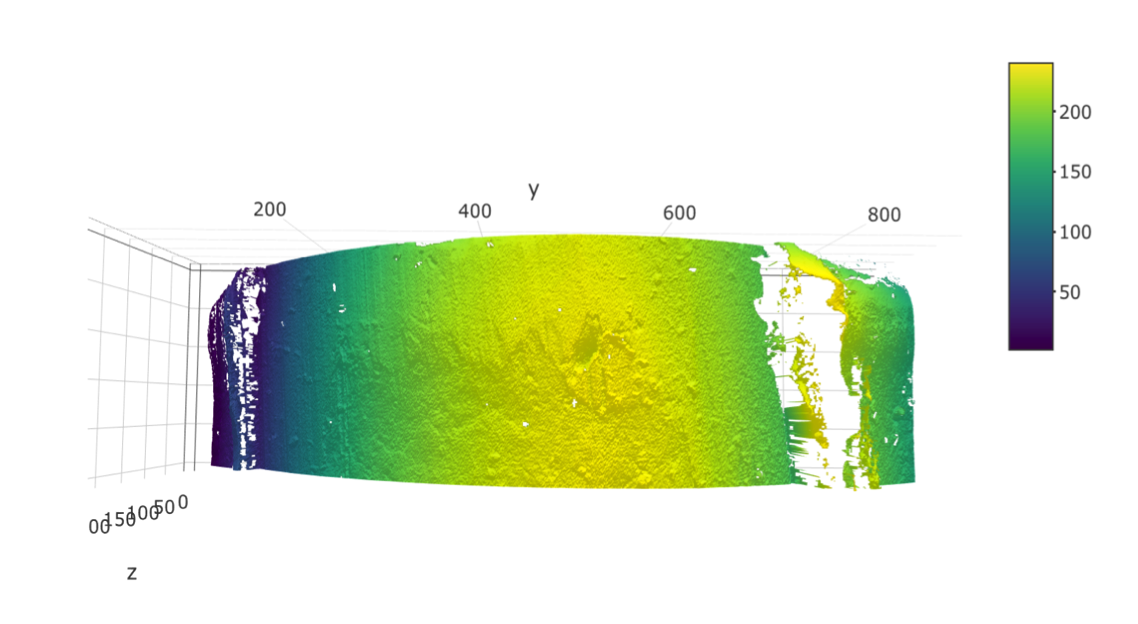
\includegraphics[width=6.25000in]{./images/3d_plot_top.png}
\caption{Visualization of 3D data collected through high resolution
scanning of a land engraved area. Striations on the surface of the
object can be seen by viewing this data from ``above'', as presented
here.}
\end{figure}

Image-analysis algorithms, while flexible enough to focus on a variety
of patterns in the data, should mainly focus on comparison of striation
marks and related characteristics that can be calculated. This focus
addresses two concerns associated with introducing an automated
approach. First, it ensures physical interpretability of characteristics
that are calculated from the gathered data. Further, researchers are
able to directly compare the visual process examiners use to an
automated method which is rooted in the same principles; for example,
when a data-based Consecutively Matching Striae (CMS) measure is
calculated as part of the algorithm. This striation-focused approach
suggests mainly utilizing horizontal slices of the 3D scan, called
crosscuts, that capture the striation pattern horizontally across the
surface, as seen in Figure 3.

\begin{figure}
\centering
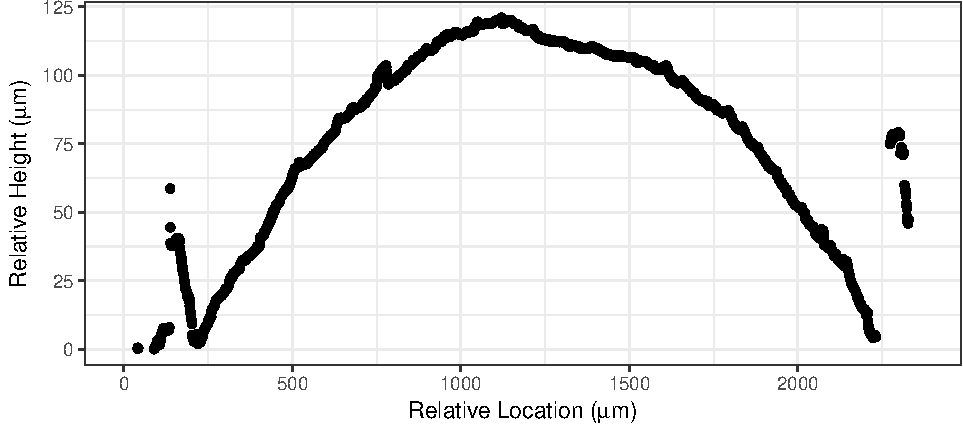
\includegraphics{writeup_files/figure-latex/unnamed-chunk-2-1.pdf}
\caption{Single crosscut of 3D bullet land data. The main data
structure, located in the center, is comprised of the land engraved
area. The groove engraved areas occur to the left and right sides of the
crosscut.}
\end{figure}

The final data consists of 2D crosscuts gathered from 3D imaging. The
height values in the crosscuts were averaged over several crosscuts
spaced out along the 3D image. This ensures predicted locations will be
relatively applicable across the depth of the bullet. Two scans were
removed from consideration due to data quality concerns, leaving 208
individual crosscuts which function as the dataset.

\section{Methodology}

The nature of the data structure is such that much of the variability
found within the data is due to the global structure of the physical
object; that is, the curve of a bullet. Since the goal is to identify
where the global data structure changes (where the shoulder location
is), methods need to be able to separate out the LEA structure from the
GEA structure. This can most effectively be accomplished by fitting a
line to the curve of the bullet and analyzing the pattern of deviations
from that curve. That is, fitting a statistical model to the curve of
the bullet and examining the residual values.

Due to two competing structures in the data, the ideal statistical model
is one which treats the secondary structure of the GEA as outlying data
and fits the curve of the LEA alone. We examine two methods for fitting
the LEA structure that are based on robust statistical methods. While
the two approaches differ in methodology, they are both rooted in the
ability to mitigate undue influence caused by outlying data.

\subsection{Robust Linear Models}

Due to the curved nature of the bullet, a quadratic linear model is a
good candidate model. Linear models are based on minimizing the vertical
squared distance between each data point and a fitted line. This means
that if there are data points in unusual places, a linear model will fit
a line that is pulled towards outlying data in order to minimize the
overall sum of squared distances. In this particular data environment,
the fitted curve can be easily influenced by GEA data, as is seen in
Figure 4.

The robust approach under the linear model framework focuses on
minimizing the least absolute deviations. This method of minimization is
less influenced by possibly large outlying values present in the GEA
data. Due to the overwhelming majority of data being from the LEA
structure, minimizing the least absolute deviations will favor fitting
the LEA structure and allowing GEA data to have large residual values.
This is preferable to the traditional linear model, which corrects for
the presence of GEA data by compromising between the two competing
structures, and does not fit either structure appropriately. A striking
example of the difference in results from these two model frameworks is
seen in Figure 4.

\begin{figure}
\centering
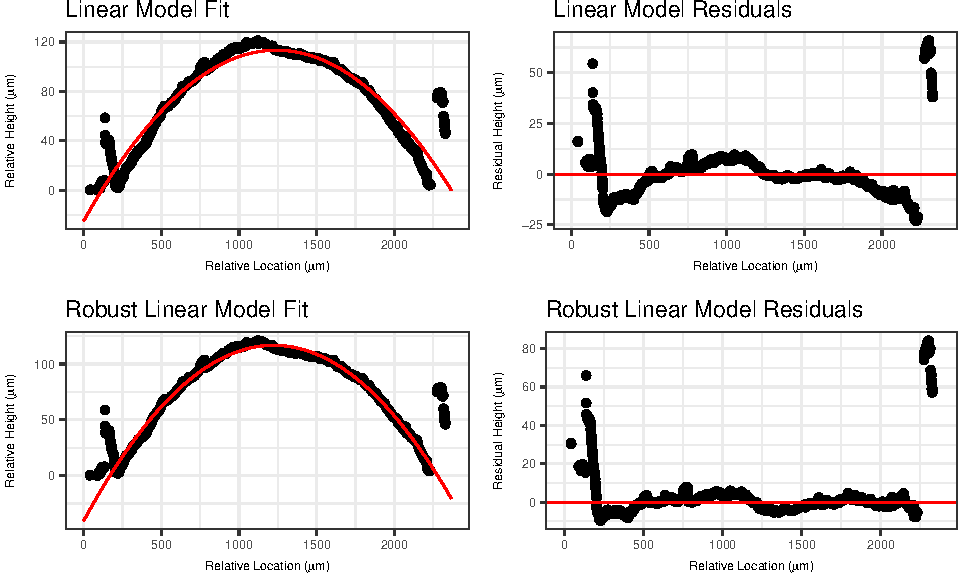
\includegraphics{writeup_files/figure-latex/unnamed-chunk-3-1.pdf}
\caption{Example of a quadratic linear model fit and resulting residuals
(top) compared to a robust quadratic linear model fit and residuals
(bottom) for a single crosscut. The robust model is able to more
effectively capture the curved structure of the LEA without being
influenced by the GEA.}
\end{figure}

Once a model has been fit for each crosscut, residual values are
calculated. The model, having fit the structure of the LEA, results in
small residuals scattered around zero in the LEA zone, and larger,
mostly positive residuals in the GEA zones. Thus, the magnitudes of the
residuals themselves can serve as one indicator of whether a data point
is part of the LEA structure or the GEA structure. A cutoff value for
the magnitude to separate the residuals from the two zones can be
employed. Investigating the median absolute residual (MAR) value, a
cutoff that works well to distinguish between GEA and LEA data residuals
on the Hamby set 44 is 4*MAR. Any residual value larger than 4 times the
median absolute residual value can be seen as a ``large'' residual.

Shoulder location predictions are calculated for each crosscut in the
following manner:\\

\begin{enumerate}
\item Fit a robust linear model of order 2 (i.e., quadratic) to the averaged crosscut.   
\item Calculate a residual value for each data point on the crosscut.  
\item Calculate the median absolute residual (MAR) for the crosscut.  
\item Remove all data points on the crosscut whose absolute residual value is greater than 4*MAR.  
\item Identify the range of the remaining X values - these are the predicted shoulder locations for that crosscut.   
\end{enumerate}

\subsection{Robust LOESS}

Locally weighted regression, known as LOESS, is an approach that is not
restricted by the need for perfect quadratic curvature. This is
advantageous when working with bullets, as it is unrealistic to expect a
flawless circular shape to remain after the bullet has been subjected to
the forces of a gun barrel and striae have been impressed upon it.

LOESS fits many models to small subsets of the data and combines them
into one non-parametric fit of the data, rather than focusing on the
overall structure of the data. This allows for greater flexibility.
However, it also means that LOESS models are affected by GEA structures
in a much more unpredictable manner. A model fitted on a subset of data
that mainly falls in the GEA structure will look vastly different than
another model fit with data from the LEA. This results in a combined
prediction that misrepresents much of the data near one or both shoulder
locations (see Figure 6).

Just as the nature of LOESS models differs from traditional linear
models, the robust approach must differ too. Robust LOESS utilizes an
iterative process focused on re-weighting \citep[see][]{Cleveland1}.
First, an initial LOESS fit is created. This is followed by a step which
gives smaller weights to data points with high residual values, and a
subsequent LOESS fit with new weights applied. The down-weighting of
values with high residual values slowly reduces the influence of a
secondary structure within the data; here, the GEA data. This iterative
process results in a non-parametric fit to the LEA structure that treats
GEA data as less important, which is desirable in this context.

While robust LOESS methods are more flexible than robust linear models,
a model that is accurately fit to the LEA structure will result in the
same expected residual structure as with robust linear models: positive
and negative residuals scattered around zero in the LEA zone, and
positive, possibly large residuals in the GEA zones. A similar approach
as with the robust linear model cutoff value to distinguish between
``large'' residual values and reasonable ones; however, because this
model is more flexible and fits more closely to the specific data at
hand, our cutoff will be lower. A cutoff that performs well on the Hamby
set 44 is twice the median absolute residual (2*MAR).

\begin{figure}
\centering
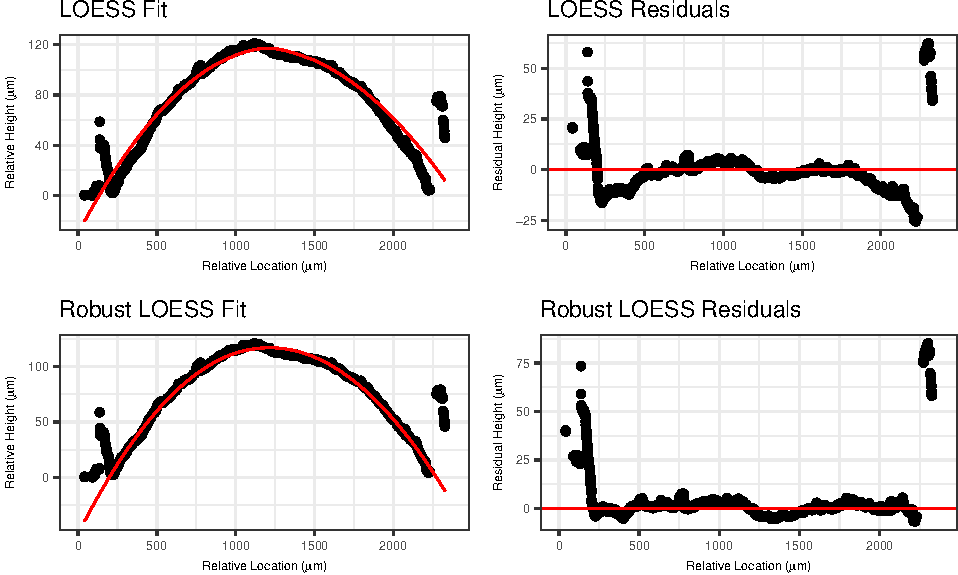
\includegraphics{writeup_files/figure-latex/unnamed-chunk-4-1.pdf}
\caption{Example of a LOESS model fit and residuals (top) compared to a
robust LOESS model fit and residuals (bottom) for a single crosscut. The
robust model is again able to more effectively capture the curved
structure of the LEA without being influenced by the GEA.}
\end{figure}

Shoulder location predictions are calculated for each crosscut in the
following manner:

\begin{enumerate}
\item Fit a robust LOESS model with a span of 1 to the averaged crosscut. This is fit using the `locfit.robust` function in the `locfit` package in R.
\item Calculate a residual value for each data point on the crosscut.  
\item Calculate the median absolute residual (MAR) for the crosscut.  
\item Remove all data points on the crosscut whose absolute residual value is greater than 2*MAR.  
\item Identify the range of the remaining Y values - these are the predicted shoulder locations for that crosscut.   
\end{enumerate}

\section{Results}

In order to assess the accuracy of these predictions, we take a unique
approach. To calculate a quantitative measure for the overall
performance of predictions, we first manually identified ``ground
truth'' shoulder locations.

The numerical comparison of predicted and manually identified locations
presents a troubling issue; raw distance metrics can misrepresent the
true character of a prediction's accuracy. For example, take a predicted
shoulder location that falls 10 data points away from the manually
identified shoulder location. This 10-point difference could be caused
by noise in the data, missing data points, or simply the miniscule scale
of the data. After all, a span of 10 data points represents only 6.45
microns in physical space. Alternatively, a distance of 10 points could
actually be 10 points that are part of the groove engraved area, and
thus are being incorrectly identified and could later cause problems.

Thus, a more relevant measure is to investigate the residual values that
fall between the predicted and manually identified shoulder location.
This penalizes shoulder location predictions that are too far out to the
side and leave GEA data in the main structure. Because the robust LOESS
most reliably approximates the curved shape of the bullet land due to
its flexibility, we want to use residual values resulting from that
model to assess final performance of all methods. Residual values from
the GEA will not necessarily be uniformly large, but are expected to be
positive as their structure and the modeling technique dictates that
they would fall above the fitted line from robust LOESS.

Given this assumption, even a 10-point difference can quickly add to a
large residual sum if we are dealing with all positive values, as
opposed to a 10-point difference within the land engraved area that will
be balanced out by the presence of both positive and negative residual
values and remain closer to zero.

For this reason, gathering the sum of residuals between the predicted
location and the manually identified location is appropriate. This
residual sum is referred to as an ``inaccuracy score'' for which higher
values indicate a higher level of inaccuracy. An inaccuracy score was
calculated separately for the left and right predictions for each
crosscut in the data set.

Of interest are the distributions of these inaccuracy scores across all
208 lands used in the study. A distribution that has a smaller spread
and is close to zero is ideal; this suggests many of the predicted
shoulder locations are very close to the manually identified locations,
and predictions are removing many of the outlying GEA points. A
distribution with a wider spread or many high, outlying inaccuracy
scores suggests a greater degree of uncertainty and inaccuracy for a
particular method.

It is important to note that different results are expected for the left
and right shoulder locations. Within Hamby set 44, almost all scans have
a well-defined left groove. Left here is defined as visually left on the
scan; this is the side the scan begins on, so a well-defined distinction
between GEA and LEA is expected. Often, a less clear distinction is seen
on the right side of the scan, with sometimes no apparent shoulder
location visible. For this reason it is preferable to separate the left
and right for visual inspection of results; a method could excel on one
side but fall short on another.

\textbf{Once results are re-run on fresh manual identifications, there
may be discussion here of differences between left and right seen in our
data.}

\begin{figure}
\centering
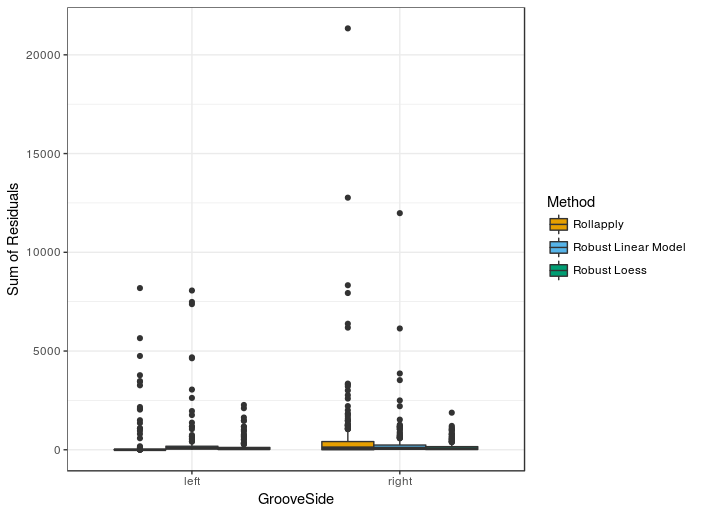
\includegraphics{./images/afte_results.png}
\caption{Distribution of inaccuracy scores for data smoothing method,
robust linear model method, and robust LOESS method, separated by left
and right shoulder locations. A tight distribution with few high values
indicates good performance across the LEAs in the data set.}
\end{figure}

\section{Conclusions}

Both the robust linear model and robust LOESS approaches outperform
currently implemented solutions based on data smoothers. Of the two, the
robust LOESS approach clearly outperforms the robust linear model. This
hierarchy of performance is well within expectation given the strength
of robust approaches in general as well as the flexibility of LOESS
applied to this data type. Robust LOESS also readily handles variation
introduced in the process of translating the physical bullet into a 3D
object. If there is too much variability in how the bullet is placed
relative to the plane of reference \textbf{(??)} on the microscope,
crosscuts can have tilted shapes relative to the x-axis which a
quadratic linear model would fail to address. In these situations, LOESS
excels.

While the cutoff values presented work well on Hamby set 44, additional
cross-validation will need to be implemented on a variety of bullet
types. Depth of striae, physical size of bullet due to caliber, and
non-traditional rifling techniques may require some alterations to this
cutoff value. In addition, a study of the effect of implementing a
robust LOESS data pre-processing strategy on overall automated
image-analysis methods will need to be addressed. Due to increased
accuracy of predicted shoulder locations, the authors expect an increase
in accuracy in bullet matching algorithms. However, this will need to be
validated on a variety of data sets prior to implementation without
human intervention in the automated process.

\section{References}

\bibliographystyle{jfs-authoryear}
\bibliography{bibliography.bib}

\end{document}
